\documentclass[a4paper, 10pt]{article}

\title{MOSIG M1 Visual Computing TP4}
\date{}
\author{Gilchrist N'dri \and Quoc-Trung Vuong}

\usepackage[utf8]{inputenc}
\usepackage{listings}
\usepackage{color}
\usepackage{amsmath}
\usepackage{graphicx}
\usepackage{geometry}

\geometry{a4paper, portrait, margin=1in}

\definecolor{dkgreen}{rgb}{0,0.6,0}
\definecolor{gray}{rgb}{0.5,0.5,0.5}
\definecolor{mauve}{rgb}{0.58,0,0.82}

\lstset{
  language=C,
  showstringspaces=false,
  columns=flexible,
  basicstyle={\small\ttfamily},
  numbers=none,
  numberstyle=\tiny\color{gray},
  keywordstyle=\color{blue},
  commentstyle=\color{dkgreen},
  stringstyle=\color{mauve},
  otherkeywords={},
  breaklines=true,
  breakatwhitespace=true,
  tabsize=2
}

\begin{document}
\maketitle

\paragraph{Test subject} All illustrations used in this report are results of the respective operation applied on the boat image \texttt{boat\_noise.pgm} from TP2. The image is filtered using binomial filter with size of $3\times3$ for 5 times.
\begin{figure}[!htb]
\centering
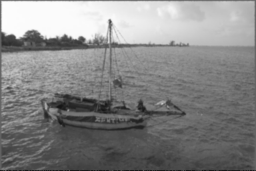
\includegraphics[width=256px]{boat3x3_5.png}
\caption{Test subject}
\label{fig-subject}
\end{figure}


\section{Gradient}
\subsection{Approximate gradient using Sobel operator}
\paragraph{} We apply Sobel operator ($3\times3$) on the image to obtain its approximate gradient of each pixel along each axis: horizontal ($x$) and vertical ($y$)
\subsubsection{$x$-axis}
\paragraph{} The approximate gradient on each pixel $(m,n)$ is computed by the following formula:
\begin{equation}
I_x(m,n) = \sum_{i=m-1}^{m+1}\sum_{j=n-1}^{n+1}{h_x(i-(m-1),j-(n-1)) * I(i,j)}
\end{equation}
with coefficient $h_x$ being:
\begin{equation}
h_x = \frac{1}{4} * \left[
\begin{matrix}
-1 & 0 & 1 \\
-2 & 0 & 2 \\
-1 & 0 & 1
\end{matrix}
\right]
\end{equation}

For pixels on each border, we set the gradient to be $0$.

\paragraph{Implementation}
We use the same function for computing gradient on both direction for each pixel, with the last argument specifying the mask to apply filter on.
\begin{lstlisting}[frame=single]
float gradient_1d(gray *map, int i, int j, int rows, int cols, float *mask) {
  if (i - 1 < 0 || i + 1 >= rows || j - 1 < 0 || j + 1 >= cols) {
    return 0;
  }

  float val = 0.0f;
  for (int i1 = i - 1; i1 <= i + 1; i1++) {
    for (int i2 = j - 1; i2 <= j + 1; i2++) {
      int mask_index = (i1 - i + 1) * 3 + (i2 - j + 1);
      int img_index = i1 * cols + i2;
      val += (float) map[img_index] * mask[mask_index];
    }
  }
  return val;
}
\end{lstlisting}

The function to obtain Sobel filter mask for $x$-axis:
\begin{lstlisting}[frame=single]
float *sobel_mask_x() {
  float *mask = malloc(sizeof(float) * 9);
  mask[0] = -1.0f / 4;
  mask[1] = 0;
  mask[2] = 1.0f / 4;
  mask[3] = -2.0f / 4;
  mask[4] = 0;
  mask[5] = 2.0f / 4;
  mask[6] = -1.0f / 4;
  mask[7] = 0;
  mask[8] = 1.0f / 4;
  return mask;
}
\end{lstlisting}

Put them together to compute the whole image gradient:
\begin{lstlisting}[frame=single]
float *grad_x_image = malloc(cols * rows * sizeof(float));
for (i = 0; i < rows; i++) {
  for (j = 0; j < cols; j++) {
    grad_x_image[i * cols + j] = gradient_1d(graymap, i, j, rows, cols, sobel_mask_x());
  }
}
\end{lstlisting}

\subsubsection{$y$-axis}
\paragraph{} The approximate gradient on each pixel $(m,n)$ is computed by the following formula:
\begin{equation}
I_y(m,n) = \sum_{i=m-1}^{m+1}\sum_{j=n-1}^{n+1}{h_y(i-(m-1),j-(n-1)) * I(i,j)}
\end{equation}
with coefficient $h_y$ being:
\begin{equation}
h_y = \frac{1}{4} * \left[
\begin{matrix}
-1 & -2 & -1 \\
0 & 0 & 0 \\
1 & 2 & 1
\end{matrix}
\right]
\end{equation}

The gradient on border pixels is set to $0$.

\paragraph{Implementation}
We apply the same method as with Sobel filter on $x$-axis. The filter mask is replaced with:
\begin{lstlisting}[frame=single]
float *sobel_mask_y() {
  float *mask = malloc(sizeof(float) * 9);
  mask[0] = -1.0f / 4;
  mask[1] = -2.0f / 4;
  mask[2] = -1.0f / 4;
  mask[3] = 0;
  mask[4] = 0;
  mask[5] = 0;
  mask[6] = 1.0f / 4;
  mask[7] = 2.0f / 4;
  mask[8] = 1.0f / 4;
  return mask;
}
\end{lstlisting}

\subsection{Gradient images}
\paragraph{} The gradient values $I_x$ and $I_y$ can be either positive or negative, and we are not sure how large its absolute value can be. Therefore, we need to apply stretching (or shrinking) to translate their value range to $(0, 255)$ for display purpose.

The function below takes an array of real numbers and translate them to $(0, maxval)$ scale:
\begin{lstlisting}[frame=single]
gray *float_to_image(float *gradient, int rows, int cols) {
  float min_mag = 0;
  float max_mag = 0;
  for (int i=0; i<rows * cols; i++) {
    if (gradient[i] > max_mag) {
      max_mag = gradient[i];
    }
    if (gradient[i] < min_mag) {
      min_mag = gradient[i];
    }
  }

  gray *out = malloc(rows * cols * sizeof(gray));
  for (int i=0; i<rows; i++) {
    for(int j=0; j<cols; j++) {
      out[i * cols + j] = (gray) ((gradient[i * cols + j] - min_mag) / (max_mag - min_mag) * maxval);
    }
  }
  return out;
}
\end{lstlisting}

\paragraph{Results} The illustrations can be seen on figure \ref{fig-gradient}.

\begin{figure}[!htb]
\centering
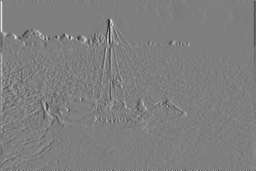
\includegraphics[width=192px]{boat3x3_5_grad_x.png}
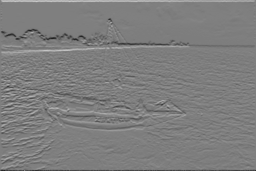
\includegraphics[width=192px]{boat3x3_5_grad_y.png}
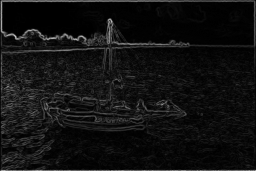
\includegraphics[width=192px]{boat3x3_5_grad_mag.png}
\caption{From left to right, gradient x, gradient y, gradient magnitude of the test subject}
\label{fig-gradient}
\end{figure}


\section{Interest Point Detection}
\subsection{Gradient $I^2_x$, $I^2_y$, $I_{xy}$}
We use the following functions computing $I^2_x$, $I^2_y$, and $I_{x,y}$ for each pixel $(i, j)$:

\begin{lstlisting}[frame=single]
float gradient_x2(gray *map, int i, int j, int rows, int cols) {
  float gradient_x = gradient_1d(map, i, j, rows, cols, sobel_x);
  return gradient_x * gradient_x;
}
\end{lstlisting}

\begin{lstlisting}[frame=single]
float gradient_y2(gray *map, int i, int j, int rows, int cols) {
  float gradient_y = gradient_1d(map, i, j, rows, cols, sobel_y);
  return gradient_y * gradient_y;
}
\end{lstlisting}

\begin{lstlisting}[frame=single]
float gradient_xy(gray *map, int i, int j, int rows, int cols) {
  float gradient_x = gradient_1d(map, i, j, rows, cols, sobel_x);
  float gradient_y = gradient_1d(map, i, j, rows, cols, sobel_y);
  return gradient_x * gradient_y;
}
\end{lstlisting}

\paragraph{Results} The illustrations can be seen on figure \ref{fig-gradient-square}.

\begin{figure}[!htb]
\centering
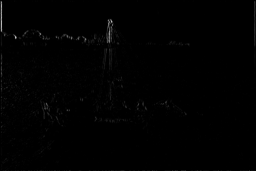
\includegraphics[width=192px]{boat3x3_5_grad_x2.png}
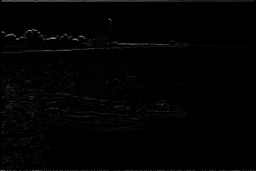
\includegraphics[width=192px]{boat3x3_5_grad_y2.png}
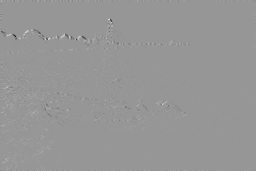
\includegraphics[width=192px]{boat3x3_5_grad_xy.png}
\caption{From left to right, gradient $I_x^2$, gradient $I_y^2$, gradient $I_{xy}$ of the test subject}
\label{fig-gradient-square}
\end{figure}





\begin{lstlisting}[frame=single]
\end{lstlisting}
\end{document}